% !TEX root = DesignDocument.tex


\chapter{Prototypes}

%%This chapter is for recording each prototype developed.  It is a historical record of what you accomplished in 464/465.   This should be organized according to Sprints.  It should have the basic description of the sprint deliverable and what was accomplished.  Screen shots, photos, captures from video, etc should be used.  

\section{Sprint 1 Prototype}
Sprint 1 was almost entirely research and forming/signing the software contract.  There was a rough draft of the gallery room that would be considered a prototype, however the design team neglected to take screenshots of it.
\subsection{Deliverable}
The deliverable for this sprint was the signed software contract and the gallery room in the Unreal Engine.
\subsection{Backlog}
	\begin{enumerate}
	\item Finalize gallery room
	\item Movement prototypes
	\item Frame and place each painting
	\item Text descriptions
	\item Alternate environment
	\end{enumerate}
\subsection{Success/Fail}
Succeeded in rendering the room in the correct dimensions as well as integrating the Oculus Rift headset into the Unreal Engine. This will allow the user to see in the environment later on in development.

\section{Sprint 2 Prototype}
Sprint 2 focused mainly on the two movement methods.  Every painting was placed in the environment as well making the gallery room more complete.  
\subsection{Deliverable}
The two movement methods: Free movement, and On-rails movement.
\begin{figure}
	\caption{This is the free movement blueprint code}
	\centering
	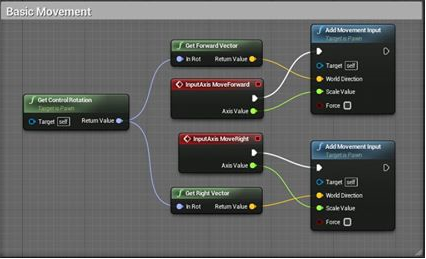
\includegraphics[scale=1.0]{SprintReports/Sprint2/basicMovement.png}
\end{figure}
\begin{figure}
	\caption{The first half of the on-rails blueprint code}
	\centering
	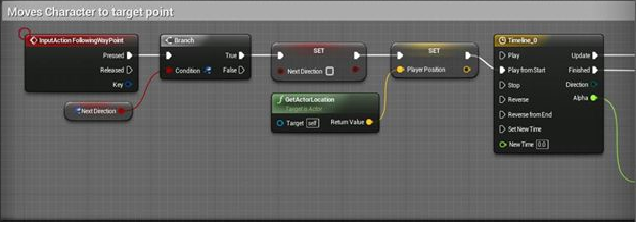
\includegraphics[scale=1.0]{SprintReports/Sprint2/moveToPoint.png}
\end{figure}
\begin{figure}
	\caption{The second half of the on-rails blueprint code}
	\centering
	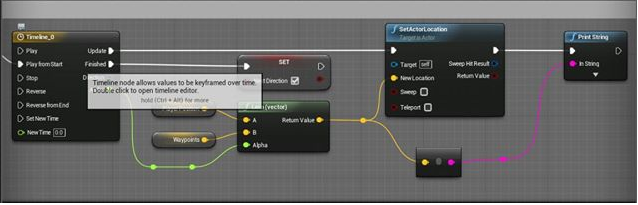
\includegraphics[scale=1.0]{SprintReports/Sprint2/moveToPoint2.png}
\end{figure}
\subsection{Backlog}
	\begin{enumerate}
	\item Finalize gallery textures and lighting
	\item Frame and place remaining paintings
	\item Text descriptions
	\item Alternate environments
	\end{enumerate}
\subsection{Success/Fail}
Succeeded in finishing both movement methods, ahead of schedule as well as some lighting and textures for the gallery room.  Failed to have all of the paintings included in the gallery.

\section{Sprint 3 Prototype}
Sprint 3 was where the development team tested the movement methods, as well as finished placing the paintings and most of the lights.  This is also where the entire on-rails tour was finalized.
\subsection{Deliverable}
Blueprints of the on-rails tour will be shown as well as the array of coordinates used in the tour.  Pictures of the room will also be displayed showing what it looks like at this point in the project.

\begin{figure}
	\caption{The first half of the on-rails tour blueprint}
	\centering
	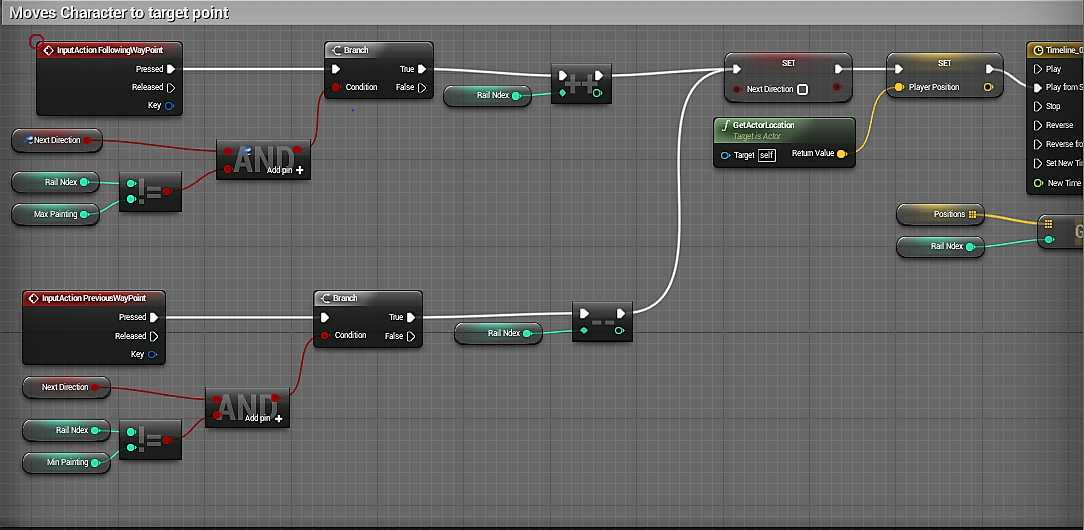
\includegraphics[scale=0.5]{SprintReports/Sprint3/WayMove1.png}
\end{figure}

\begin{figure}
	\caption{The second half of the on-rails tour blueprint}
	\centering
	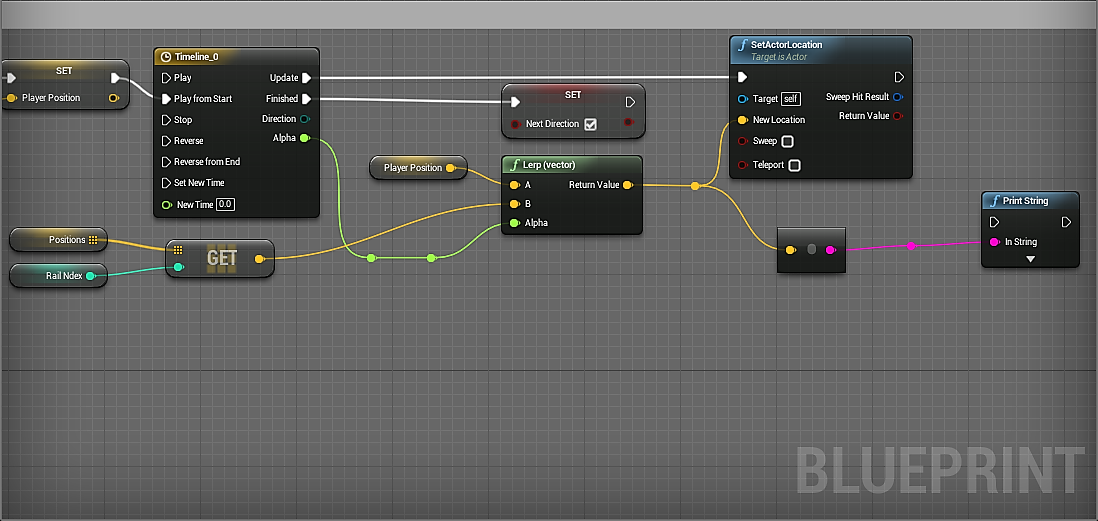
\includegraphics[scale=0.5]{SprintReports/Sprint3/WayMove2.png}
\end{figure}

\begin{figure}
	\caption{A section of the coordinates array used in the on-rails tour}
	\centering
	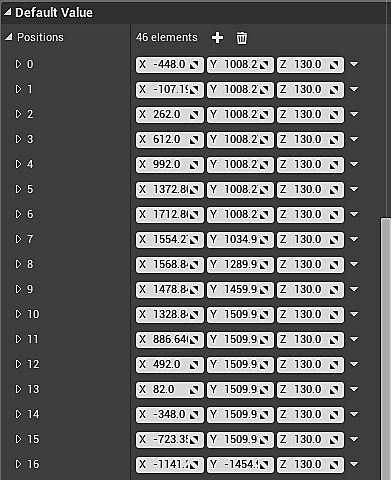
\includegraphics[scale=0.5]{SprintReports/Sprint3/Waypoint.png}
\end{figure}

\begin{figure}
	\caption{The gallery so far with more light}
	\centering
	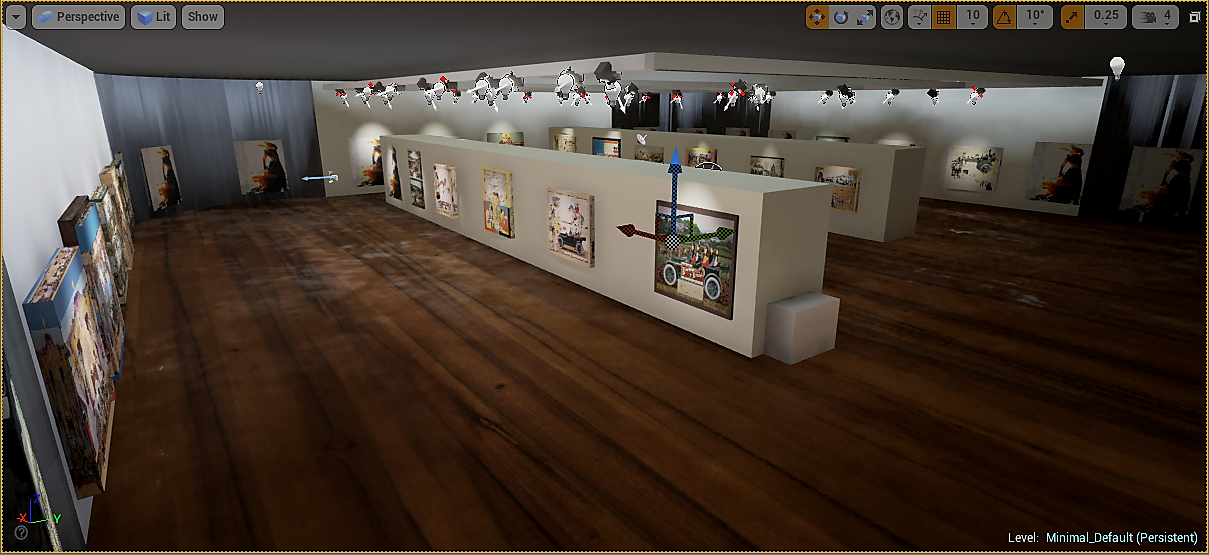
\includegraphics[scale=0.5]{SprintReports/Sprint3/Example1.png}
\end{figure}

\begin{figure}
	\caption{The gallery from a darker corner}
	\centering
	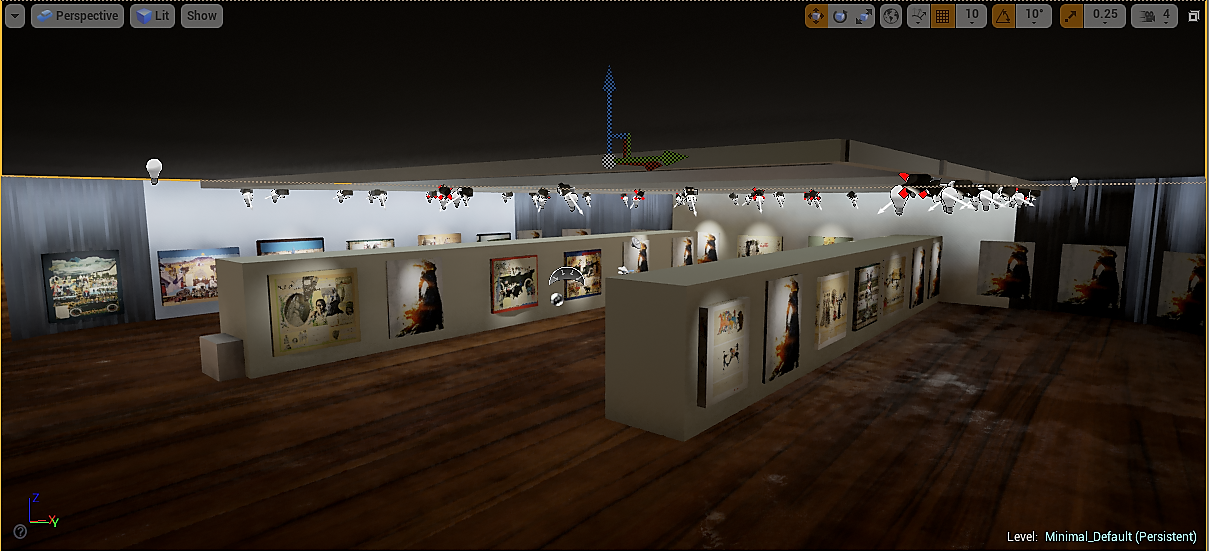
\includegraphics[scale=0.5]{SprintReports/Sprint3/Example2.png}
\end{figure}
\subsection{Backlog}
\begin{enumerate}
	\item Finalize gallery textures and lighting
	\item Text Descriptions
	\item Alternate environments
\end{enumerate}
\subsection{Success/Fail}
Succeeded in implementing the on-rails tour of all available paintings.  Failed in having the gallery finished.

\section{Sprint 4 Prototype}
\subsection{Deliverable}
\subsection{Backlog}
\subsection{Success/Fail}

\section{Sprint 5 Prototype}
\subsection{Deliverable}
\subsection{Backlog}
\subsection{Success/Fail}

